\documentclass[sigconf]{acmart}

%% Remove ACM Reference Format and citation information
\settopmatter{printacmref=false} % Removes citation information below abstract
\renewcommand\footnotetextcopyrightpermission[1]{} % Removes footnote with conference information in first column

\acmConference{Data Security and Privacy in the Age of AI} % Conference name
\acmYear{Spring 2025} % Year

\usepackage{graphicx} % Required for inserting images
\usepackage{xcolor}

% \usepackage{authblk}

% \usepackage{fullpage}

\newcommand{\todo}[1]{\textcolor{red}{\textbf{TODO:} #1}}

\title{Membership Inference for Proprietary Large Language Models}

%% Authors and affiliations
\author{Muhammad Hamza}
\email{muhamza@vt.edu}
\affiliation{%
  \institution{Virginia Polytechnic Institute and State University}
  \city{Blacksburg}
  \state{VA}
  \country{USA}
}

\author{Syed Talal Hasan}
\email{syedtalal@vt.edu}
\affiliation{%
  \institution{Virginia Polytechnic Institute and State University}
  \city{Blacksburg}
  \state{VA}
  \country{USA}
}

\author{Minh Hoang Tran}
\email{tran189@vt.edu}
\affiliation{%
  \institution{Virginia Polytechnic Institute and State University}
  \city{Blacksburg}
  \state{VA}
  \country{USA}
}

\renewcommand{\shortauthors}{Hamza, Talal, Hoang}

\begin{document}


% \begin{abstract}
% add abstract here    
% \end{abstract}

\keywords{Membership Inference, Large Language Models, Data Privacy}

\maketitle


\section{Introduction}

% \todo{do this at the end, lets cite the news articles too for cases etc}

Large Language Models (LLMs) have become ubiquitous, offering impressive capabilities in generating text for applications ranging from chatbots to creative content. However, training these models often involves vast datasets that may include both publicly available information and private or proprietary data. This practice raises serious concerns about copyright infringement and privacy violations. In many cases, individuals or organizations may need to verify whether their specific data was included in a model’s training set.

Recently, there have been multiple lawsuits against OpenAI brought by New York Times and other authors for copyright infringement \cite{key}. There are other key lawsuits against Anthropic, Cohere and Perplexity as well on different aspects, however, one thing they all have in common is the allegation of the use of copyrighted and proprietary data without authorization. All of these organizations that have created these foundation models deny the use of private data and claim they only used 'public information' for training. 

Membership inference involves determining whether a specific piece of data was included in a model’s training set. For instance, \cite{neurons_read_your_book} proposed a method for performing document-level membership inference on large language models. Similarly, \cite{extracting_training_data_llm} shows that an adversary can extract verbatim sequences from a model’s training data, highlighting potential privacy concerns. 

Traditional approaches to membership inference often rely on analyzing the probabilities a model assigns to the next word in a sequence, based on the assumption that models tend to assign higher probabilities to sequences they encountered during training. While effective, these techniques generally require fine-grained access to the model’s internal outputs, such as raw probability distributions. However, applying these methods becomes significantly more difficult when dealing with proprietary commercial models, like OpenAI’s GPT and Claude’s Sonnet series, that do not expose such internal information.

This project aims to investigate whether we can use model outputs as a signal to identify whether it has seen a given document during training or not, based on similarity. We use the difference in similarity as a measure to find how the LLM would behave differently with data it has seen vs that it has not. We explore the use of the cosine semantic similarity using all-MiniLM-L6-v2 sentence embedding within Membership Inference tasks. We demonstrate that prompting models to generate documents within its training dataset results in higher semantic similarity scores against the original document compared to doing the same with documents not within the model's training set.

\section{Background}
\subsection{Large Language Models}
Large language models (LLMs) are a new advancement in Natural Language Processing (NLP). At their core, LLMs take in a sequence of words (tokens), and attempt to generate the most likely subsequent words (next-token-prediction). In order to do this in a manner generate tokens that are not only grammatically but also (mostly) informationally correct, LLMs require extremely large corpuses of training data \cite{stochastic_parrots}.

Ever since their commercial debut, LLMs have exploded into a multi-trillion dollar industry [insert\_citation]. This has subsequently raised concerns about security and intellectual property regarding what works were included within the training datasets various LLMs\cite{bloomberg_artist_suit}. As most commercial models do not disclose their training data\cite{gpt4_technical_report}, the task of determine whether or not a text had been used in the training of an LLM - membership inference - is of growing importance.

\subsection{Membership Inference Techniques}

Previous works have explored avenues for determining the membership status of a particular text in a model's dataset. \cite{neurons_read_your_book} described a probabilistic method of determining document-level membership, in which the normalized probability distribution of how often a token appears in the generated text is compared against its distribution in the original document. Documents whose generated texts have a similar token probability distribution to the original are thus classified to be part of the training data.

On the other hand, rather than determining membership on a document level, \cite{extracting_training_data_llm} described a method to extract an LLM's knowledge of any arbitrary string of tokens by having the model generate a large amount of text, and then measuring the perplexity of various token sequences. High perplexity sequences are then selected for manual evaluation to see if they exist elsewhere online.


% Actually this may be part of related works. Talk about techniques used for models where we can access the produced probability distribution. This is something not available for propiratiary ones.
% I can't find any attacks in either the online literature or in the mentioned papers that describe an attack based on open weights. -H

% Also mention stuff like perplexity/trainging loss as a way for membership inference. This too is not available to us for proprietary models. A paper was talking about this (you'll have to check).
% Yeah it's the Carlini paper. -H

% \todo{Hoang please add this}

\section{Membership Inference}

This section outlines our proposed methodologies for performing membership inference on proprietary large language models (LLMs).

Due to the restricted nature of proprietary models, our access is limited to a small set of external parameters—such as temperature, system prompts, and input text --- while internal components like model weights and token-level probability distributions remain inaccessible. Consequently, our approach relies solely on analyzing the model’s generated outputs.

The central hypothesis underlying our techniques is that if a model encountered a document during training, it may retain some semantic understanding of that document. Accordingly, we aim to infer membership by evaluating the degree of semantic similarity between the model’s generated completion and the original document.

To assess semantic similarity, we use the cosine similarity of sentence embeddings of the model’s generated output and ground truth. For sentence embeddings, we use the \texttt{all-MiniLM-L6-v2} model, as it is open-source, lightweight, and easily deployable on standard hardware, while still providing competitive performance on semantic similarity tasks.

% This project aims to develop a membership inference technique tailored to proprietary large language models (LLMs), which often restrict access to internal representations such as probability outputs or hidden states. A straightforward approach might involve comparing the model’s generated text to a reference text on a word-by-word basis. However, such methods are easily defeated by paraphrasing, synonym substitution, and other variations in phrasing. To address this, we propose a more robust alternative: measuring the semantic similarity (cosine similarity) between the model’s output and the reference text. By leveraging sentence embeddings, we can assess how closely the generated response aligns with the original input at a semantic level rather than relying on exact word matches.

% To implement this approach, we design an evaluation procedure that compares semantic similarity across membership and non-membership datasets. For each text sample, we begin by splitting the document approximately in half. We then prompt GPT-4o with the first half and allow it to generate the continuation until it reaches a length roughly equal to the second half. Once generated, we compare the semantic similarity score between GPT-4o’s output and the original withheld portion of the text using sentence embeddings. This process is repeated across both the membership and non-membership datasets.

\subsection{What's next}

\begin{figure*}[htp]
  \centering
  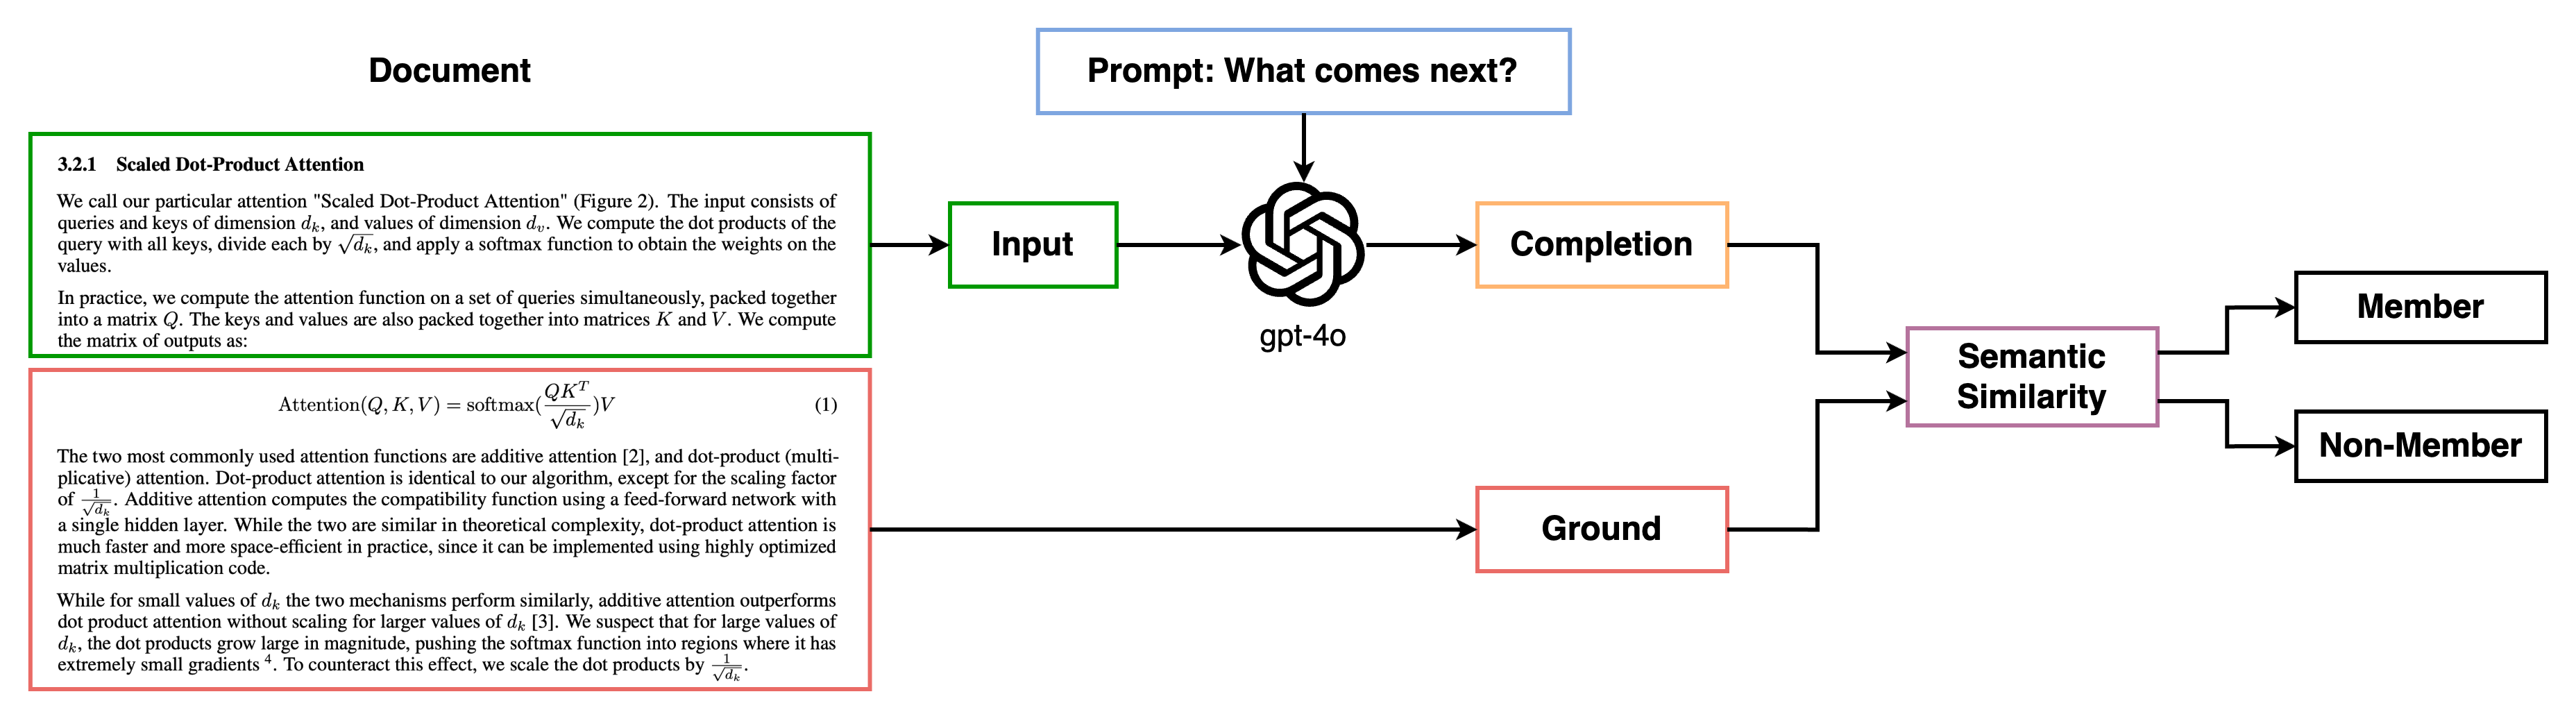
\includegraphics[width=\textwidth]{figures/completion.drawio.png}
    \caption{An overview of the "What's Next" technique for membership inference}
    \label{fig:completion}
\end{figure*}

We propose a technique called "What’s Next", which leverages the model’s capability as a next-word predictor. The central intuition is that a model’s output is influenced by the data it has encountered during training. Therefore, by analyzing how a model completes a given input, we can infer whether the associated document was likely included in its training dataset.

The workflow of this technique is illustrated in Figure~\ref{fig:completion}.  To determine if a document is part of the training data, we divide it into two segments: the first half serves as input to the model, and the second half acts as the ground truth for evaluation. We prompt the model with the first segment and request it to generate a continuation. The generated output is then compared to the original second segment to assess semantic alignment. This comparison is performed using sentence embeddings and cosine similarity. If the document was present in the model’s training set, we expect the generated continuation to exhibit high semantic similarity to the ground truth; otherwise, the similarity should be significantly lower.

\subsection{Fill in the blanks}

\begin{figure*}[htp]
  \centering
  % scale the image to the full text width:
  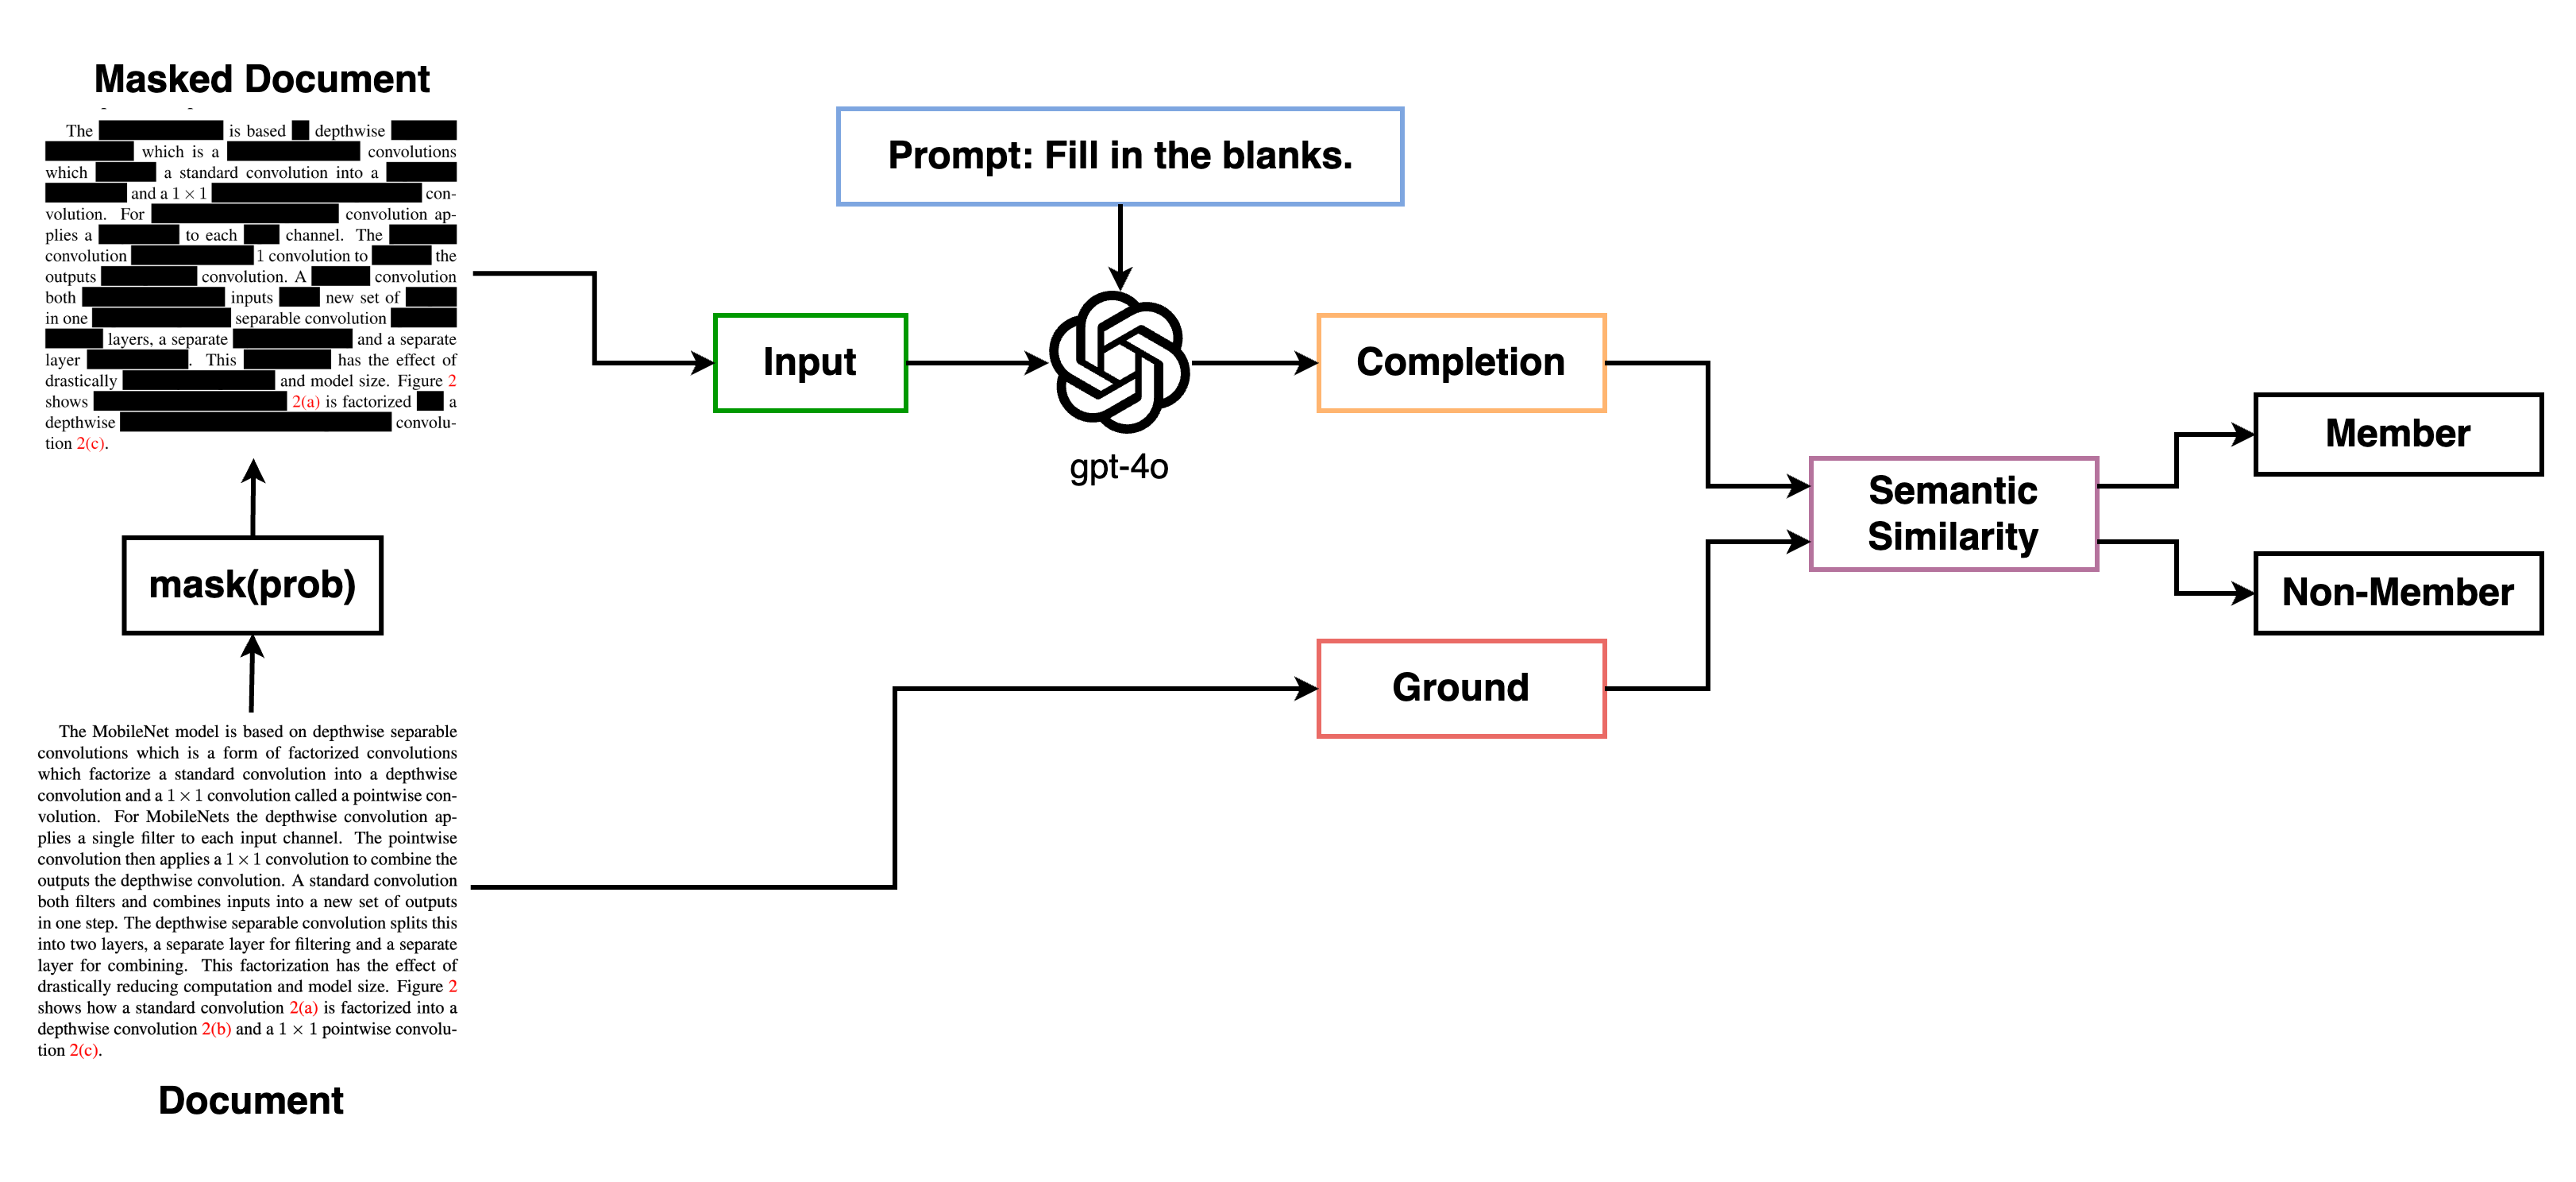
\includegraphics[width=\textwidth]{figures/masking.drawio.png}
    \caption{An overview of the "Fill in the blanks" technique for membership inference}
    \label{fig:fill-in-the-blanks}
\end{figure*}

We propose a technique called "Fill in the Blank", which evaluates a model’s memory of a document to determine whether it was likely included in the training data. The central intuition is similar to that of the previous technique — a model’s memory is influenced by the data it encountered during training. If a model has seen a particular document during training, it should be able to accurately complete a "fill in the blanks" style task based on that document. 

The workflow of this technique is illustrated in Figure~\ref{fig:fill-in-the-blanks}. To evaluate the membership status of a given document, we randomly replace a subset of words with the token \texttt{<MASK>}, based on a fixed masking probability. This produces a version of the document with substantial portions removed. We then prompt the model to fill in the masked tokens, effectively reconstructing the original content. The model’s output is compared to the original document to assess how accurately it recovers the masked words. However, a direct word-by-word comparison is often too rigid, as the model may generate synonyms or semantically similar alternatives rather than exact matches. To address this, we compare the model’s output to the original text using sentence embeddings and cosine similarity --- a high similarity score suggests membership; a low score suggests non-membership.

\section{Datasets}

To evaluate the performance of our proposed membership inference technique, we construct two distinct datasets—one for membership inference, containing items that were \textit{likely} part of the model’s training data, and one for non-membership inference, consisting of items that were not included in the training data. Our method is based on the assumption that if a model has seen a document during training, it will be more capable of generating content that is semantically similar to that document. Conversely, if the document was not part of the training set, the generated output should exhibit lower semantic similarity.

To construct the membership and non-membership datasets, we rely on the model’s training data cutoff date. Our experiments primarily target \texttt{gpt-2024-08-06}, the GPT-4o model with the training cutoff date of August 6, 2024. We assume that any publicly available content created before this date could have been included in the model’s training data, and is therefore treated as part of the membership dataset. Conversely, content published after the cutoff is assumed to be unseen by the model and is used to form the non-membership dataset.

Following this intuition, we collect data from two content categories: academic papers and news articles. These categories were chosen based on the novelty and originality of the information they typically present. We argue that both academic publications and news reports often contain newly produced, domain-specific information that is unlikely to be replicated elsewhere before publication. This characteristic is essential for membership inference, as the technique depends on the uniqueness of the evaluated content. If a document’s content is not original --- e.g., it has been adapted or copied from other public sources --- the model may have encountered the information through alternate means, undermining the accuracy of our membership inference.

Our final dataset consists of 100 documents for each content category. For both academic papers and news articles, we include 50 samples in the membership set and 50 in the non-membership set. A summary of the dataset is provided in Table~\ref{tab:dataset}.


\begin{table}[ht]
  \centering
  \begin{tabular}{lcc}
    \hline
    & Member & Non-Member \\
    \hline
    Academic Papers & 50 & 50 \\
    News            & 50 & 50 \\
    \hline
  \end{tabular}
  \caption{Counts of items in the dataset}
  \label{tab:dataset}
\end{table}


\subsection{Academic Papers}

We collected academic papers from arXiv, an open-access repository widely used in the scientific community. ArXiv was chosen because it is open-source, and is frequently used as a data source in training large language models.

For the membership dataset, we selected machine learning papers from 2018 with the highest citation counts. We used the OpenAlex API—an open-source catalog of scientific papers—to retrieve and rank these papers. Since they were published well before the GPT-4o's training cutoff in August 2024 and are both public and widely cited, it is likely that they were part of the model’s training data.

For the non-membership dataset, we used machine learning papers uploaded to arXiv in May 2025. Because these papers were published after the training cutoff date, they are unlikely to have been included in the model’s training set and thus serve as reliable non-membership examples.

\subsection{News}

We collected news article from the BBC, Reuters, and USA Today. These 3 publications were chosen as they are 3 of the most popular non-paywall English-language news outlets, thus ensuring a high likelihood of their articles being included within the training data of various LLMs.

For the membership dataset, we selected news article from 2023 - prior to GPT-4o's data cutoff date. For the non-membership set, we included news articles from 2025.


\section{Experimental Setup}

Our evaluation pipeline relies on the use of OpenAI's API that was used to run experiments on ChatGPT 4o, 4o-mini and Google Gemini. We used the system prompt to provide instructions and leveraged it to create few-shot and in-context examples as well for different experimental evaluations. In addition, we also vary different aspects of the model to evaluate their effect on the membership attack:

\begin{itemize}
    \item Temperature
    \item Context length
    \item Prompt style
    
\end{itemize}

\subsection{Temperature}

The idea of temperature was to restrict the model to produce the most likely next word instead of letting it be creative. We experimented with temperatures of 0.1, 0.3 and 0.5 to assess at what strength it produces the best results. The results of temperature exceeding 1 were the models tendency to start producing gibberish and incoherent sentences, which is expected. 

Since we were limited by the number of API calls we could make, we tested our hypothesis on a subset of data to determine the best temperature and discovered that 0.1 produced the best results. For this reason we ran all subsequent experiments using this temperature setting. 

% \subsection{Prompt Style}

% Our experiment also used different prompting styles. We initially asked it to simply complete the information from the given sequence, but this did not yield the best results. We then pivoted and adopted an instructive style for completing the information from the given context. 

% For the task on predicting the missing word in the experiment involving masks, we had initially instructed the model to predict the most probable 'word or phrase', but in the subsequent experiment, we removed the word 'phrase' from the prompt and this improved the results. This strengthened our hypothesis that certain prompts produce different and better results.


\subsection{Context Length}
 In the paper Scaling Up Membership Inference: When and How Attacks Succeed on Large Language Models \cite{arxivScalingMembership}, the authors showed that as you increase the context length, the membership attacks become more and more successful. However the authors used context of the scale $10^3$ and $10^4$ to demonstrate their results. 

 We did not have such a large-scale dataset, nor the financial resources to run experiments at that scale, however, we used the same idea at a more manageable scale and ran experiments in the context sizes of  1024, 2048 and 4096 on our academic paper dataset.

\subsection{Prompt Style}

\subsubsection{Few Shot}

For the few-shot prompting, we used one positive and one negative example from the dataset as supervision to the model. We appended the example in our base prompt to see if having a supervised example would enable the model to recognize the data from its memory or prompt it to leak membership data. We experimented with both just positive and both positive and negative examples in the prompt. 

\subsubsection{In Context}

Our next experiment was to divide the data into three parts: start, middle and end. The idea was to provide the model with surrounding context and make it predict the missing middle portion of the document. We divided the data where the first and last parts were 30\% each, while the model had to predict the 40\% of the tokens in the middle. This experiment also stems from the idea that if the model has information from both the beginning and the end of the document, it is more likely to reproduce and leak the membership data. 

\subsubsection{Iterative}

When interacting with the public interface API ChatGPT online, we discovered that a chain of prompts under different settings and refinements made the model leak or produce the complete training data from its memory. We had run this attack and were able to produce the data from the "Attention is all you need" paper, where it even produced the same citations as the original text.

This led us to use the same idea and prompt the model iteratively using a fixed prompt stating that it had failed to produce a result of sufficient quality and appending the produced result as part of its prompt for it to refine. We experimented with iterations of five and seven to see the effects of iterative prompting the model as a helper supervision to see if that causes it to leak the membership data. 

\subsubsection{Padding}

We also experimented with padding the base prompt to see how it would affect the model's predictions or if it would cause the model to leak information. We experimented with adding 500 and 1000 \texttt{<PAD>} tokens to the start and end of the base prompt. 

\section{Results}

\subsection{OpenAI GPT-4o}

\begin{table*}[]
\begin{tabular}{|c|c|c|c|}
\hline
                               & \textbf{Member F1} & \textbf{Non-member F1} & \textbf{All Classes F1} \\ \hline
\textbf{Temperature = 0.1}     & 0.65               & 0.44                   & 0.57                    \\ \hline
\textbf{Context Length = 4096} & 0.67               & 0.49                   & 0.60                    \\ \hline
\textbf{P(mask) = 0.3}         & 0.4                & 0.68                   & 0.58                    \\ \hline
\end{tabular}
\caption{F1 scores for the 3 orthogonal experiments, values chosen are represent ones that result in optimal classifier performance.}
\label{tab:gpt_f1_table}
\end{table*}

Ideally, we want to run all possible permutations of an experiment. but this is not possible because of limited compute credit. To get around this, we performed experiments on a subset of our dataset such that it's more economical. 

\subsubsection{What's Next with Temperature}

We evaluated our What's Next approach on both the news and academic paper datasets. To determine the most suitable temperature parameter for text generation, we first conducted experiments on the smaller news dataset.

\begin{figure}[htp]
  \centering
  % scale the image to the full text width:
  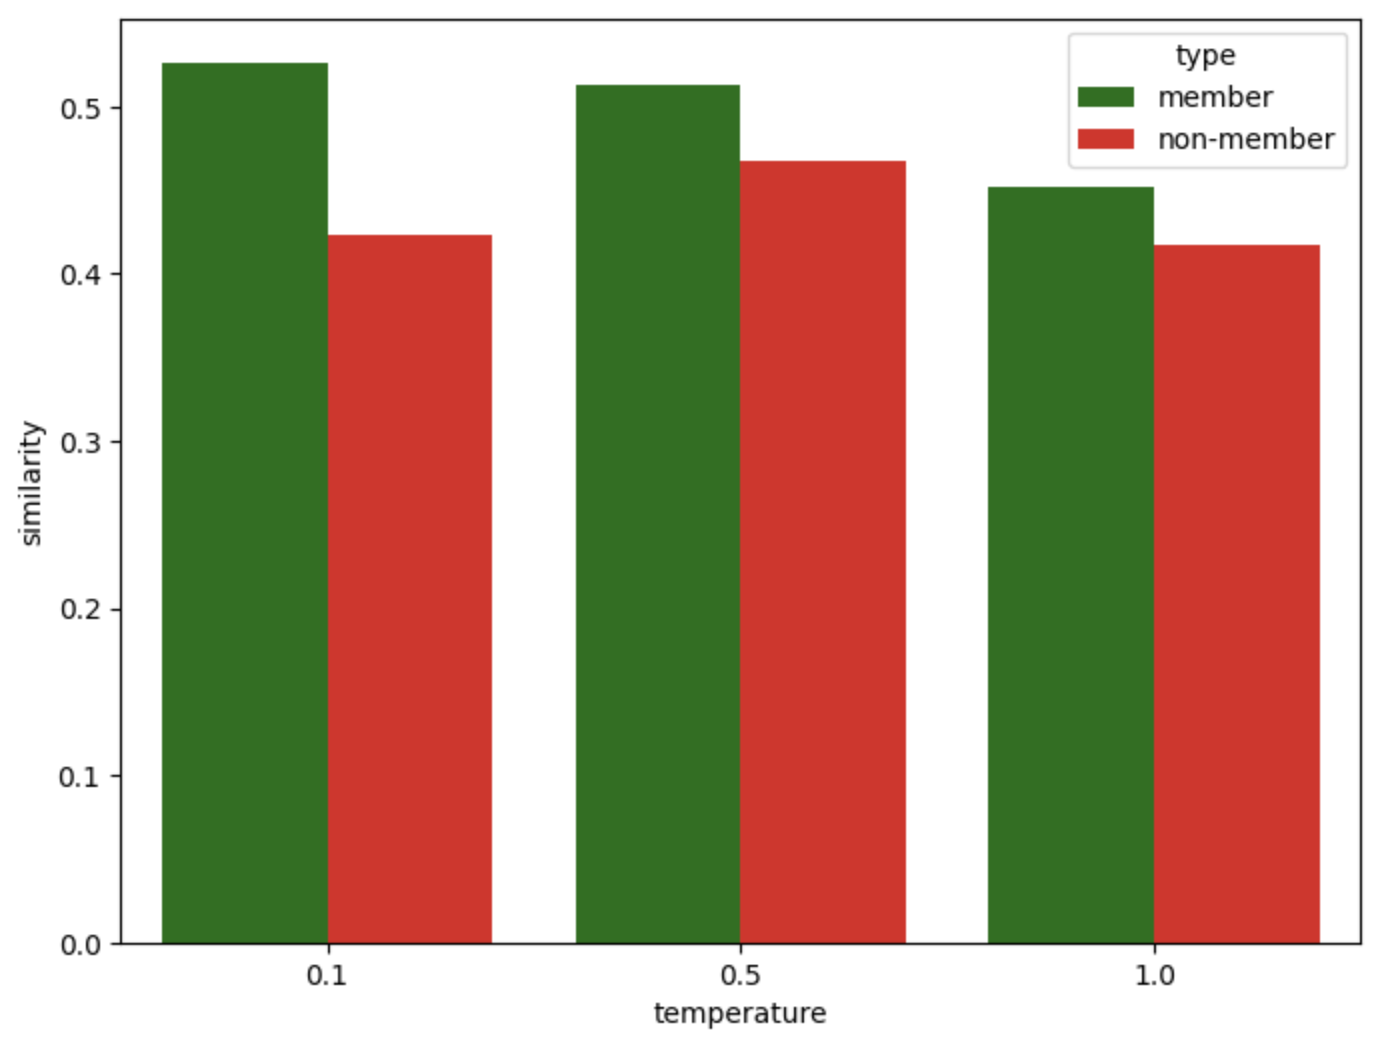
\includegraphics[width=\columnwidth]{figures/news-completion-temperature-bar.png}
    \caption{Bar chart for mean similarity scores for the 'What's Next'  technique on the news dataset over different temperatures}
    \label{fig:news-completion-temperature-bar}
\end{figure}

At lower temperatures (e.g., 0.1), the model's outputs are more deterministic, leading to higher similarity scores --- especially for member samples, which exhibit a more distinct separation from non-members. As the temperature increases, this distinction diminishes, indicating reduced membership inference capability and more stochastic generation behavior.

Figure~\ref{fig:news-completion-temperature-bar} presents the mean similarity scores for members and non-members across different temperatures tested (0.1, 0.5, and 1.0). The corresponding ROC curves are shown in Figure~\ref{fig:roc-news-completion-temperature}. Based on these curves, we selected the temperature with the highest AUC--- 0.1 --- for further analysis. Table~\ref{tab:gpt_f1_table} summarizes the classification performance at this temperature, reporting F1 scores of 0.65 for members, 0.44 for non-members, and an overall score of 0.57.

\begin{figure}[htp]
  \centering
  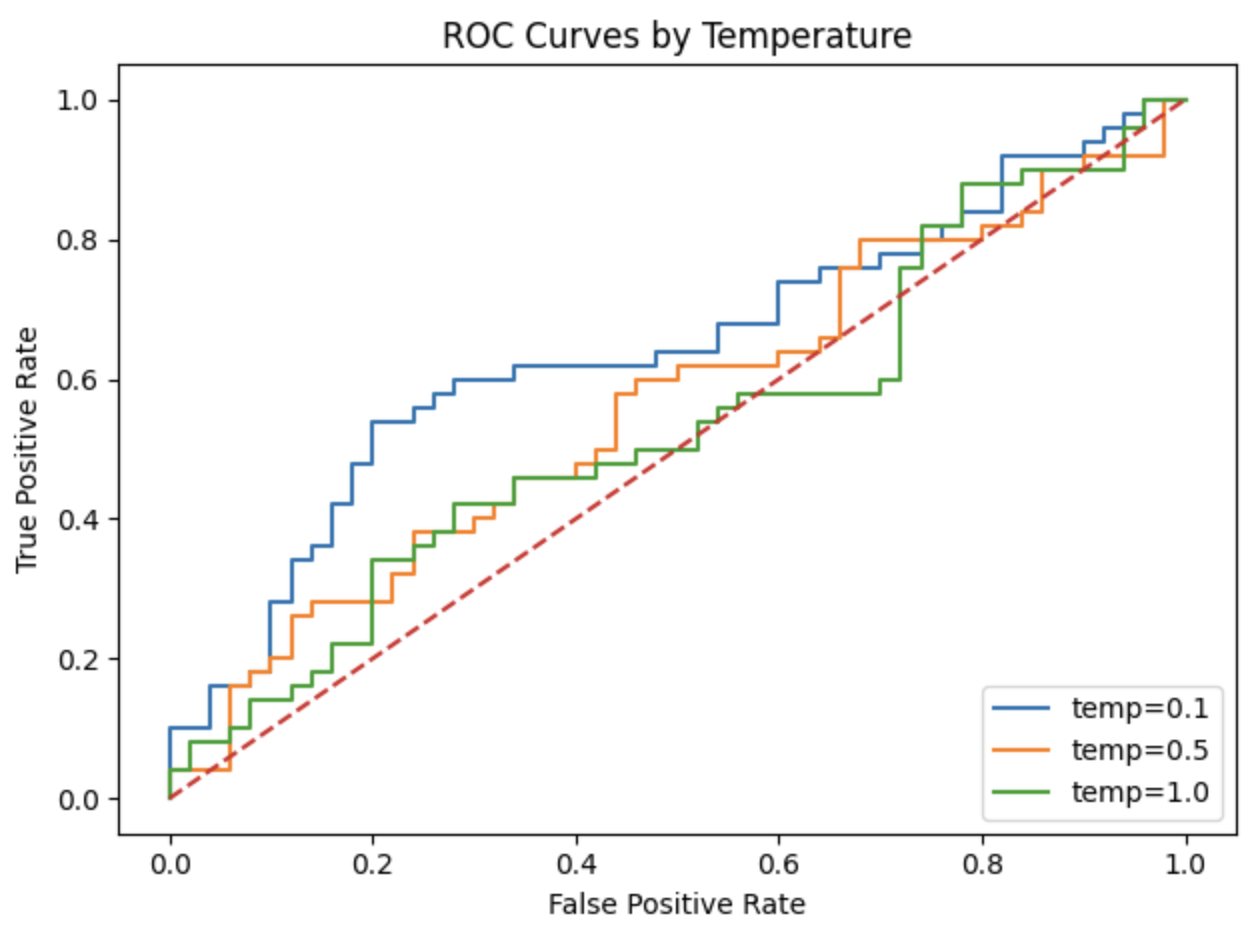
\includegraphics[width=\columnwidth]{figures/roc_gpt_temperature.png}
    \caption{Receiver-Operator curves for the 'What's Next' technique on the news dataset over different temperatures. As the temperature increases, the area under said curve decreases.}
    \label{fig:roc-news-completion-temperature}
\end{figure}

\subsubsection{What's Next with Context Length}

We also investigated whether the performance of our proposed technique is influenced by the context length of the input, as suggested by prior work~\cite{arxivScalingMembership}. Figures~\ref{fig:roc-paper-completion-context-length} and~\ref{fig:paper-completion-context-length-bar} present the Receiver-Operator curve and average similarity scores across varying context lengths (1024, 2048, and 4096 tokens).

\begin{figure}[htp]
  \centering
  % scale the image to the full text width:
  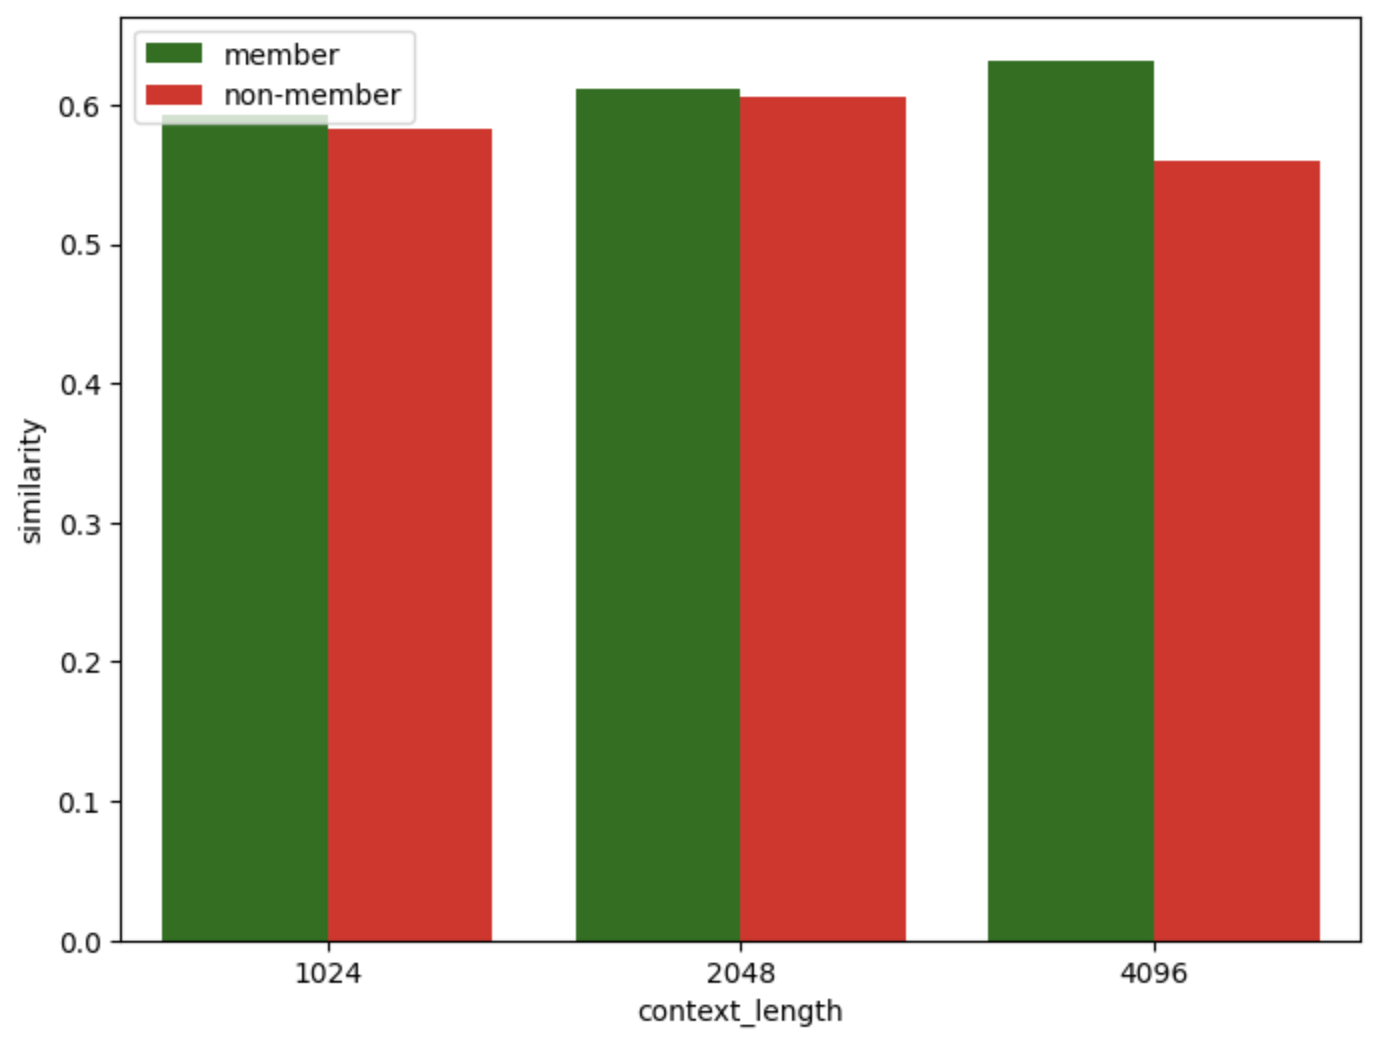
\includegraphics[width=\columnwidth]{figures/paper-completion-context-length-bar.png}
    \caption{Bar chart for mean similarity scores for the 'What's Next'  technique on the paper dataset over different context lengths}
    \label{fig:paper-completion-context-length-bar}
\end{figure}

Our results show a general trend consistent with prior studies: as the context length increases, the separation between member and non-member similarity scores becomes more pronounced. This indicates that longer contexts may strengthen the membership signal, potentially due to richer representations and more faithful continuation generation.

However, we note that the observed trends are somewhat noisy, and the performance is limited by characteristics of our dataset, as elaborated in the Limitations section. Therefore, while the results align with expectations, they should be interpreted with caution.

Figure~\ref{fig:roc-paper-completion-context-length} illustrates the ROC curves for the "What’s Next" technique applied to the paper dataset using varying context lengths (1024, 2048, and 4096 tokens). As shown, the classifier's performance improves with longer context, with the area under the ROC curve increasing accordingly. Based on this, we selected a context length of 4096 for further analysis. Table~\ref{tab:gpt_f1_table} reports the F1 scores at this setting: 0.67 for members, 0.49 for non-members, and 0.60 overall—indicating that longer context windows enhance model performance, especially for member classification.


\begin{figure}[htp]
  \centering
  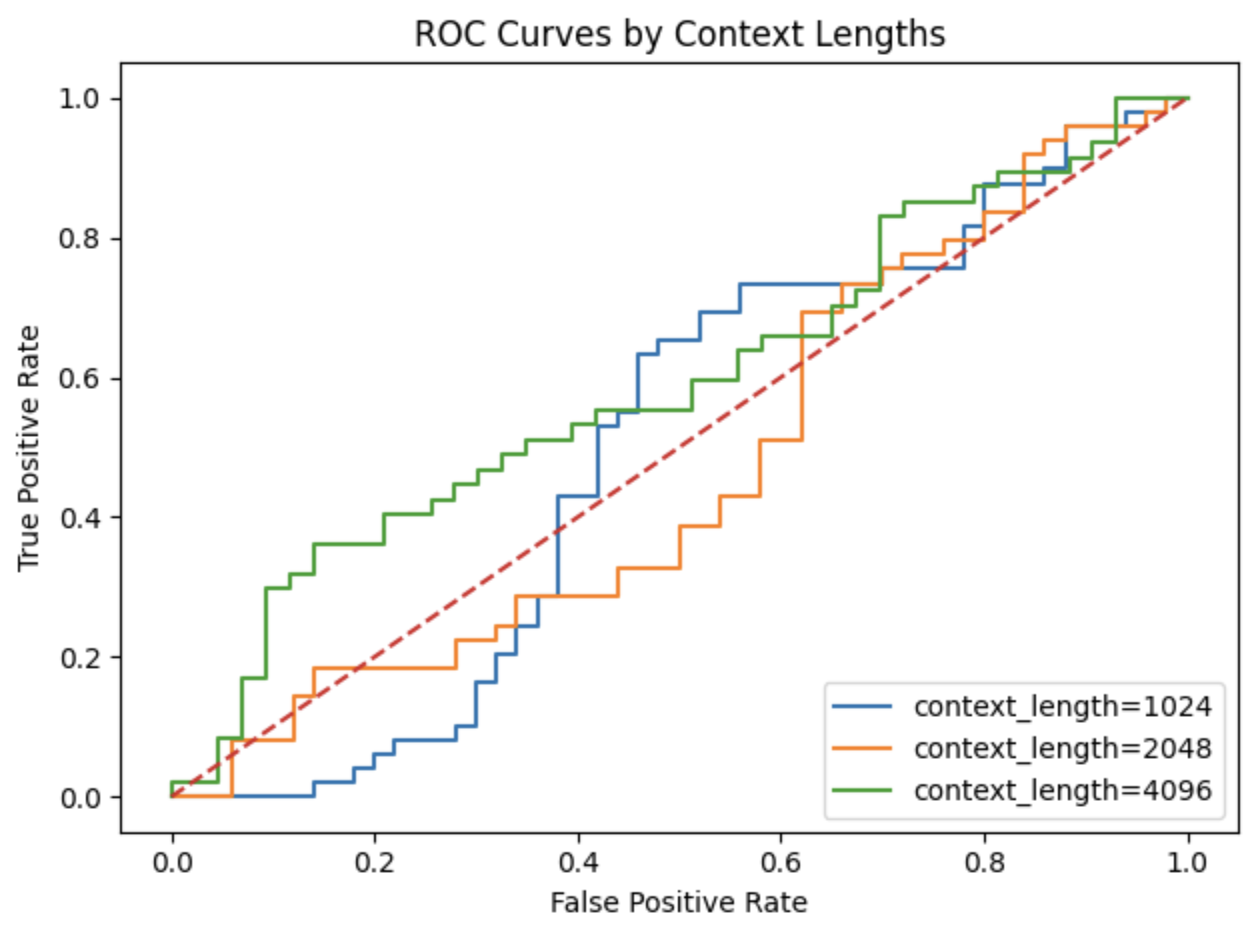
\includegraphics[width=\columnwidth]{figures/roc_gpt_context_length.png}
    \caption{Receiver-Operator curves for the 'What's Next' technique on the paper dataset over different context lengths. As the context length increases, the area under said curve increases, indicating better classifier performance.}
    \label{fig:roc-paper-completion-context-length}
\end{figure}

\subsubsection{Fill in the blanks with Mask Probabilities}

We also evaluated our fill-in-the-blanks technique using the news dataset. This dataset was chosen because it is less affected by the structural issues found in the academic paper dataset (discussed in the Limitations section), and because the news articles are generally shorter, making them more suitable for a method that leverages longer input and output spans.

To examine how the degree of masking affects performance, we varied the masking probability across three levels: 0.3, 0.4, and 0.5. Figures~\ref{fig:news-mask-prob-bar} and~\ref{fig:roc-news-mask-prob} present the average scores and Receiver-Operator curve for member and non-member samples under each setting.

\begin{figure}[htp]
  \centering
  % scale the image to the full text width:
  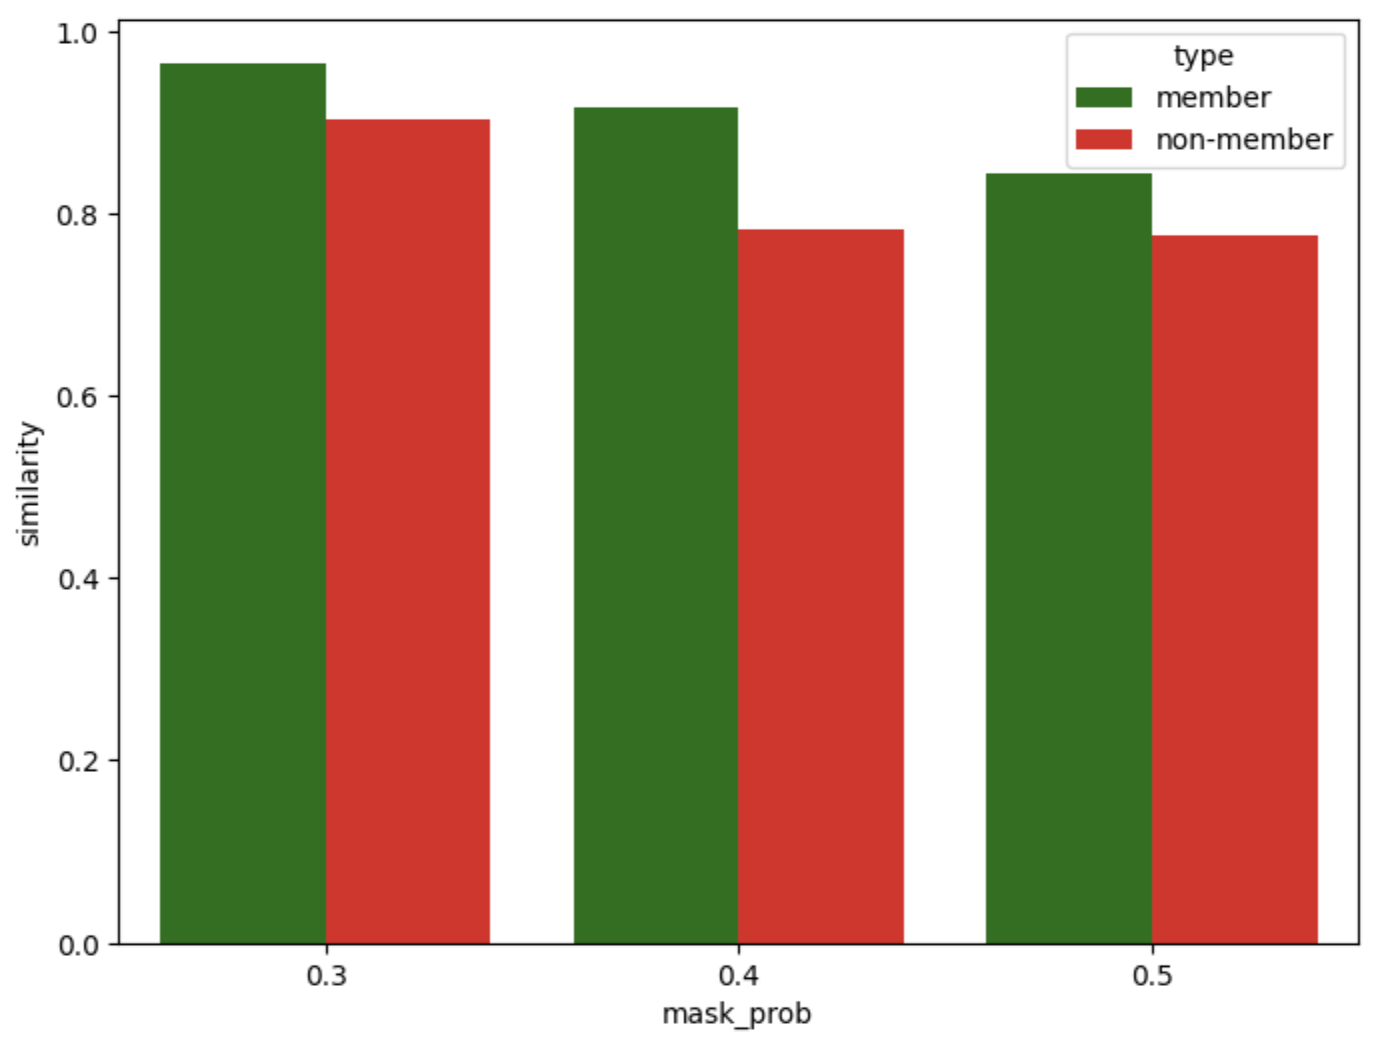
\includegraphics[width=\columnwidth]{figures/news-mask-prob-bar.png}
    \caption{Bar chart for mean similarity scores for the 'Fill in the blanks' technique on the news dataset over different masking probabilities}
    \label{fig:news-mask-prob-bar}
\end{figure}

Once again, member samples consistently show higher similarity scores than non-member samples across all masking probabilities. However, as the masking probability increases (from 0.3 to 0.5), the gap between member and non-member scores narrows, and overall similarity decreases for both groups. This is also reflected in the ROC curves. The ROC curve for 0.3 masking probability shows the best separation between member and non-member samples, while performance declines noticeably at 0.5, approaching random chance. This shows that, past 0.3, higher random masking probabilities decrease the classifier's ability to differentiate between member and non-member documents.

To quantify this, Table~\ref{tab:gpt_f1_table} reports the F1 scores at the optimal masking probability of 0.3: 0.40 for member samples, 0.68 for non-member samples, and an overall F1 score of 0.58.


These findings suggest that moderate masking offers the strongest membership signal, highlighting the importance of carefully tuning this parameter in fill-in-the-blanks style evaluations.


\begin{figure}[htp]
  \centering
  % scale the image to the full text width:
  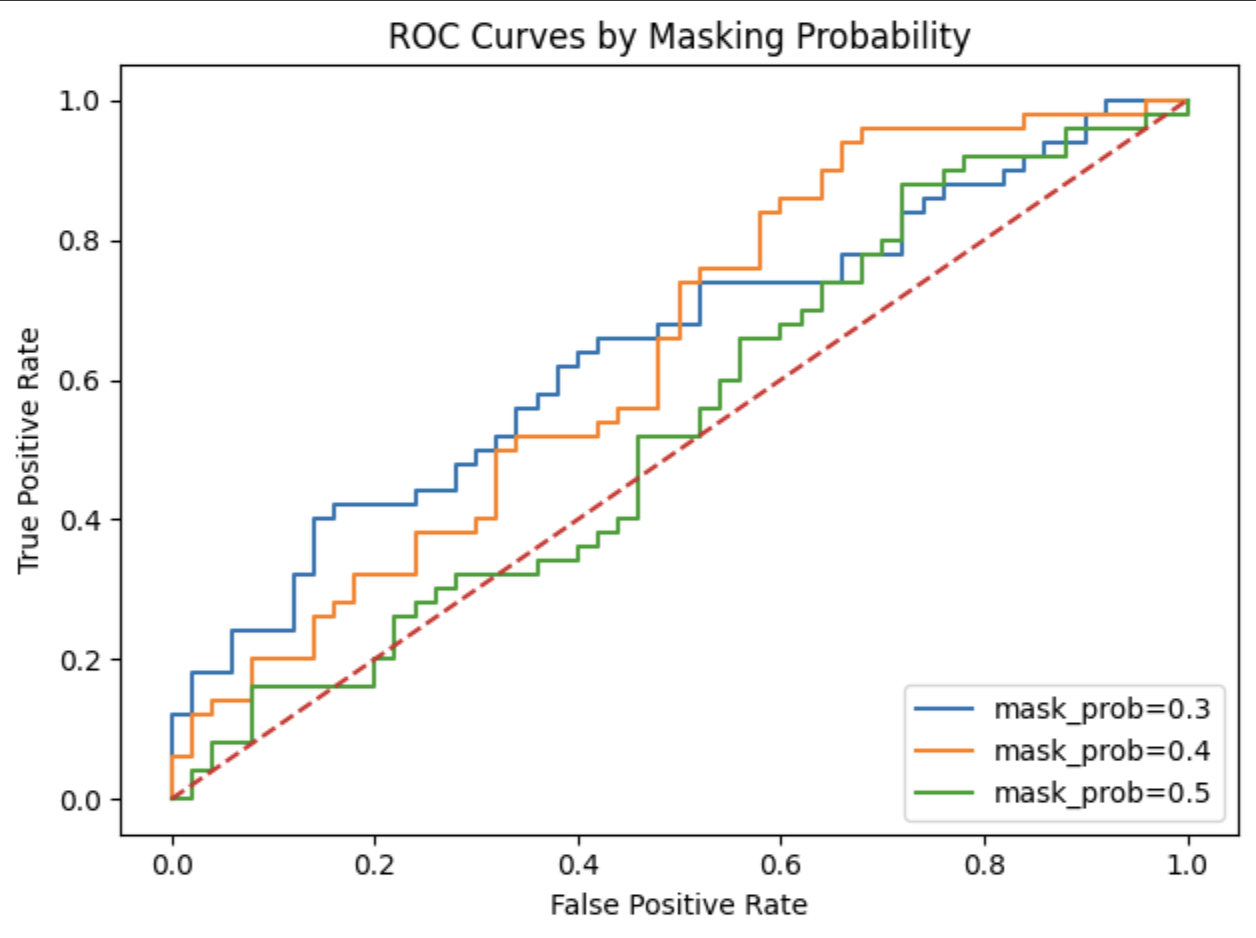
\includegraphics[width=\columnwidth]{figures/roc_gpt_masking_prob.png}
    \caption{Receiver-Operator curves for the 'Fill in the blanks' technique on the news dataset over different masking probabilities}
    \label{fig:roc-news-mask-prob}
\end{figure}


\subsection{Google Gemini 2.5 Flash}

\begin{figure*}[htp]
  \centering
  % scale the image to the full text width:
  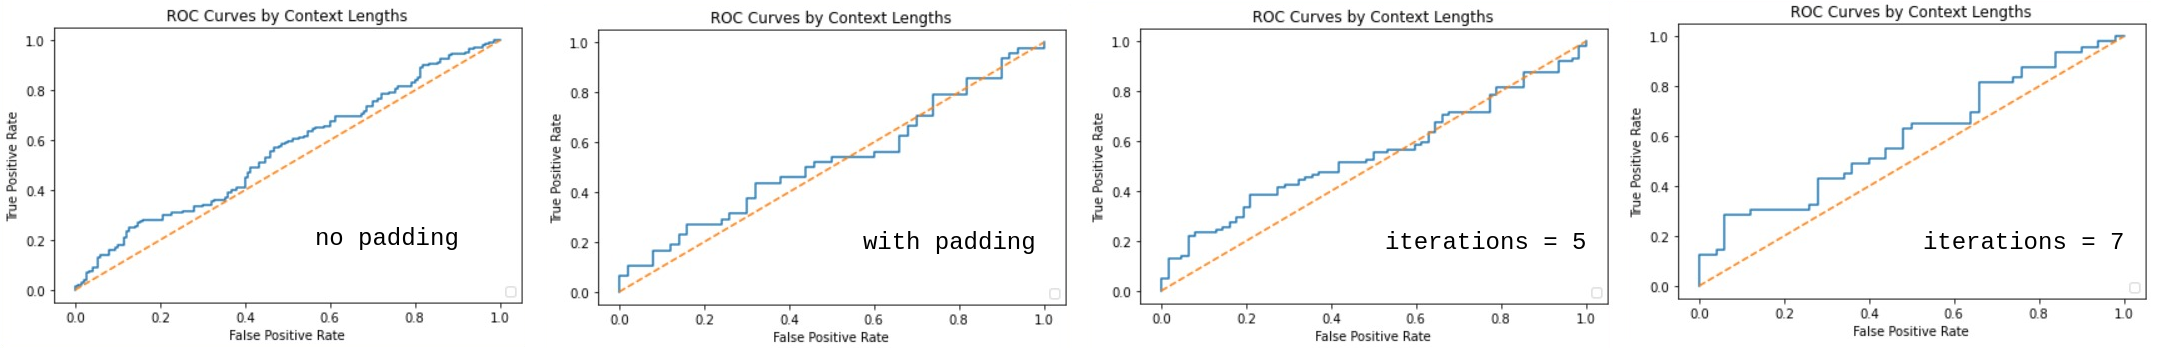
\includegraphics[width=\textwidth]{figures/gemini_collage.png}
    \caption{Receiver-Operator curves at different padding and query-iteration levels on Gemini 2.5 Flash. While the use of padding had little effect, iterating queries resulted in a greater difference in semantic similarity scores between member and non-member documents, thus increasing the classification performance.}
    \label{fig:roc_gemini_collage}
\end{figure*}

\begin{table}[]
\begin{tabular}{|c|c|c|c|}
\hline
                             & \textbf{Member} & \textbf{Non-member} & \textbf{All Classes} \\ \hline
\textbf{No Padding}          & 0.66               & 0.39                   & 0.56                    \\ \hline
\textbf{With Padding}        & 0.61               & 0.49                   & 0.56                    \\ \hline
\textbf{Iteration = 5} & 0.57               & 0.51                   & 0.54                    \\ \hline
\textbf{Iteration = 7} & 0.71               & 0.42                   & 0.62                    \\ \hline
\end{tabular}
\caption{F1 scores for the semantic-similar-based classifier with different querying parameters when operated on the Gemini model. Higher levels of padding are able to extract more learned information from the model, enabling better membership inference performance}
\label{tab:gemini_f1_table}
\end{table}

\subsubsection{Fill in the blanks}

The results for Google Gemini followed the same pattern as Chat GPT. For masking, the model produced a similarity of 0.92 for member documents and 0.9 for non-member documents when the experiment was performed on 30\% of the text in the document masked. This is a 2\% difference between member and nonmember data. This shows that having just the surrounding context is enough for the model to accurately preserve the meaning and it does not need to have seen the document to produce high similarity words. However, despite the high similarity in all experiments, member documents consistently had a higher similarity compared to nonmember documents. 


However what was surprising was that Gemini was significantly quicker in running the experiments compared to ChatGPT. The runtime efficiency was 2x compared to 4o-mini. ChatGPT took 30 minutes to run the experiment for 100 documents, while Gemini took approximately 15 minutes. 

\subsubsection{Iterative}

We ran two different experiments for iterative \textit{hand holding} one with 5 and the second with 7 iterations. If the similarity at any point exceeded a defined threshold, which we kept at 0.7 for our experiment, we exited the loop. This experiment was only possible with Gemini since it has a free tier, whereas ChatGPT does not. 

With 5 iterations, we saw a surprising result, compared to zero-shot, iteratively appending the produced prompt to the base led to a decline in similarity. In the case of 5 iterations, the average similarity score for membership documents was 0.39 and 0.33 for non membership data. With 7 iterations, we saw an improvement after decline, where the similarity for member data increased to 0.46 and 0.38 for nonmember data. The absolute average similarity difference stayed consistent but the overall average similarity increased with member data having a significantly higher similarity. 

\subsubsection{Few Shot}

We then conducted experiments with few-shot prompting. With few shot we noticed that the similarity between member and nonmember data became very similar. For member data the similarity was 0.54 and while it was 0.55 for non member data. This was surprising since we suspected that having a supervised example would cause the model to produce similar data from its training, but this was not the case. 

We then ran another experiment, where, along with a few-shot examples, we padded the base prompt with \texttt{<PAD>} tokens with 500 at the start and 500 at the end of the base prompt. This produced an interesting result, where the similarity for the member data stayed consistent at around 0.53, but the similarity of non member data decreased to 0.47. This made us aware that having more context, even if it is in the form of padding, enables better performance on data that the model has seen. 


\section{Limitations}

While our study provides important insights into membership inference on language models, several limitations must be acknowledged.

A primary limitation lies in the dataset used for evaluation. For our non-membership dataset, we collected academic papers from arXiv, published in May 2025. Although these papers were publicly released after the model’s cutoff date, it is likely that many of them draw upon previously published research or widely known ideas. Given that arXiv allows unrestricted submissions, a significant portion of the content may consist of replications, minor extensions, or reinterpretations of existing work. This undermines one of the critical assumptions of membership inference: that target documents contain domain-specific or novel information that the model could only have seen during training.

This limitation is reflected in our results, where we observed similar semantic scores for both membership and non-membership examples, specifically for the academic papers category. This suggests that the model may have encountered similar concepts or phrasing in its pretraining data, reducing our ability to distinguish true members from non-members with high confidence.

The challenge highlights the need for more sophisticated methods of constructing membership inference datasets --- ones that account for content novelty and originality. It also suggests that membership inference is most effective when applied to highly novel or proprietary data that has minimal overlap with public or previously available sources.

Additionally, our dataset was relatively small. Due to computational credit constraints, we evaluated only 50 examples from each class (member and non-member), which may not be fully representative. Larger-scale experiments would be necessary to draw more generalizable conclusions.

Another limitation is that membership inference requires making API calls to the model using input data that contains information about the content we are testing for membership. This means that the sensitive data being analyzed is effectively exfiltrated to the model provider through these API requests. Since many providers’ terms of service allow them to retain and use data submitted via APIs, there is a risk that proprietary or private content could be stored or reused by the company hosting the model. This poses additional concerns for users seeking to test models for privacy without further exposing their data.

\section{Future Work}

Our evaluation suggests that assessing a model’s memory of specific document content may offer a promising direction for more reliable membership inference. One of our initial attempts to explore this involved a fill-in-the-blank style approach, where we randomly masked portions of a document and evaluated the model’s ability to reconstruct the missing content. However, we found that random masking often failed to produce meaningful or challenging queries, limiting the effectiveness of this technique.

To build on this idea, one future direction is to use a language model to guide the masking process. Instead of masking text at random, an LLM could identify and remove key details such as named entities, technical claims, or pivotal arguments that are likely to be informative about the document’s content. The masked text can then be presented to the target model, and its predictions compared to the original document. A model that has memorized the source material would be more likely to reconstruct these details accurately.

Another promising direction involves adopting an exam-style methodology. In this setup, a comprehensive set of question–answer pairs would be generated from a given document using an LLM. These questions would then be posed to the target model, and the accuracy of its responses compared to the known answers. A model that has encountered the document during training is expected to perform significantly better, providing a clearer signal of membership.

These strategies aim to create more structured and informative probes of memorization, going beyond surface-level similarity metrics and offering finer-grained insights into what language models have retained from their training data.

\bibliographystyle{ACM-Reference-Format}
\bibliography{references}

\end{document}